\chapter{Evaluation}

\section{Demonstrate Implementations}
% Implementations: Georgiev, 2nd, Chen and own
% Implementation: Test model on dataset
% 
% Do a lines of code comparison between the different components of the different implementations
% Componetns: Data Reading, Data Loading (Trainingsetcreator) and training
% Compare to implementation without?

% Make a table of lines of code comparisons
% Make comparisons with published results

% Make observation of reused lines of code, per section
% Make observations on what would be the problems from the original implementations if other things are required

\begin{table}[ht]
	\caption{Implementations LOC comparisons} % title of Table
	\centering % used for centering table
	\begin{tabular}{p{0.2\textwidth}p{0.2\textwidth}p{0.2\textwidth}p{0.2\textwidth}p{0.2\textwidth}} % centered columns (4 columns)
		\hline\hline %inserts double horizontal lines
		Title & Total LOC  & Data Reading LOC & Data Loading LOC & Training LOC  \\ [0.5ex] % inserts table
		%heading
		\hline % inserts single horizontal line
		\citet{park2020augmenting} Without & 177  & 75 & 24 + 2 & 25 + 10  \\ \hline
		\citet{park2020augmenting} With & 101 & 1+10+78 = 89 & 8 & 3  \\ \hline
		\citet{georgiev2017low} Without & 211  & 105 & 46 & 32+30   \\ \hline
		\citet{georgiev2017low} With & 159 & 4 +46 +52+40=142 & 11 & 3 \\ \hline
		\citet{xu2019multi} Without &  & 50 & 35 & 43   \\ \hline
		\citet{xu2019multi} With & 92 & 2 + 46 + 33 & 8 & 3  \\ \hline
		Own Experiments & 364 & 8 + 52 + 78 + 46 + 33 + 49 + 40 + 33 = 339 & 15 & 8  \\ \hline
	\end{tabular}
	\label{table:LOC} % is used to refer this table in the text
\end{table}

As a way of demonstrating the way the framework offers the tools for rapid prototyping as well as reusability and extensibility, a number of implementation tasks have been made. For evaluating these aspects, the number of lines of code (LOC) for each implementation is shown, compared to implementations that have been made using pytorch, without the framework. The implementations that were chosen were multi-task set-ups described in published works, along with an implementation which is set-up to variate and analyse a number of different elements in the multi-task pipeline. Since this framework has a focus to be utilised in research, it is important to demonstrate that its results align with those reported in published results as well. The framework implementations shouldn't differ significantly from the reported results, even if they deviate due to numerous small implementation details that would unavoidably differ from the original work.\\

The results of the implementations with their LOC are given in table \ref{table:LOC}. For each implementation, things like imports, empty lines and debugging logic are ignored. Another thing that is not counted are the LOC for the actual models, as they are solely part of the PyTorch framework and their implementation would be the same without the extending framework. Each implementation without the framework covers the basic training and testing of models, which imply the three stages of the multitask deep learning pipeline mentioned earlier, namely Data Reading, Data Loading and Training. Each stage is mentioned separately in terms of LOC, to demonstrate the amount of work cutting that happens. Aside from training and evaluating models, metric calculation and visualization is handled in the same way as the framework does itself, which means calculation through sklearns metrics toolbox and visualization through TensorBoard. However, additional visualizations that are present in the framework, like those of the confusion matrices and the loss, as well as the additional storing and checkpointing that happens are not covered in those implementations. Solely the work required to replicate the original work is implemented. LOC in Data Reading are split up for each experiment that uses the framework, with the first element being the calling of the DataReader class and the subsequent elements being the separate implementations. What was included for each section goes as follows. Data Reading covers iterating over the dataset and extracting the data to a form which functions as a readable collection that can later be in turn iterated over and fed to the model. Data Loading is taking that extracted data, applying the necessary transformations so that the Training stage can simply receive and process the instances. Training then includes creating and training the model with unaltered data from the previous stage.\\

First thing which can be noted from looking at the results is the fact that Data Reading consistently comes out higher than without the framework. The reason for this is that the DataReaders do not really offer a lot of abstractions for simplifying reading datasets into usable forms for input and training of models. What they mainly do offer are quick extra quality of life features like quick reading, as well as functionalities that allow variations, which in turn can significantly reduce later work. This reduction does not only go for reusing the Data Reading structures, but is shown apparent in the significant decrease for the data loading and training sections. The extra lines of code required for the Data Reading almost exclusively come in the form of the function definitions and outputs, with the exception of having to add getter functions for the task name and the storage location that the quick reading functionalities use. \\ 

\textbf{\cite{park2020augmenting}} The first implementation \cite{park2020augmenting} targets a paper which does not actually describe a multi-task framework, but a single task one. The LOC comparisons are given in table \ref{table:LOC} and the comparison between the reported results and the framework results in \ref{table:metric}. The feature extraction - vectors outputted by the VGGish autoencoder TODO: REFERENCE - was not present yet in the framework, so had to be defined as an ExtractionMethod object following the framework. This only takes three more lines, which are function definitions. To explain the sum of LOC: the first 1 is how much LOC is required to call the complete data reading functionalities in the eventual experiment. The 10 LOC is for implementing the ExtractionMethod object, which was not covered yet by the base framework. Last LOC are for the actual implementation of extracting the data from datasets, which come close to the original required amount of LOC.\\

\citep{park2020augmenting} describes its results for two cases. In one, it has a label of leftovers which it limits to 500 instances, as to not be disproportionately present in training. In the other, it additionally removes the label 'speech' from its instances. These fall under the Data Loading section of the process, which is a feature covered by the framework. The data has to be split into a train and test set, which is also covered in the framework. These two elements explain how even single task set-ups can get significant reductions in required lines in its Data Loading process as seen in the table.  \\

Explaining the reduction for training is pretty simple, as the training loop - loading batches of data and updating the model - is covered in one function in the framework, which also covers visualization of the results. A training loop becomes as simple as creating the model, creating the Results object and inserting the necessary information in the training loop. \\

\textbf{\cite{georgiev2017low}} In the next implementation from \citep{georgiev2017low}, 4 tasks are taken from 3 datasets, but a different clip length has to be taken for the two tasks that come from the same dataset. Essentially, two different datasets must be extracted from the same dataset, with one being a subset of the other. The change in clip length can be added on the fly, using the DataReader's time\_split\_signal function, but otherwise, the same applies as before, with the framework offering little in the way of line cutting abstractions. What can be noted in the other sections, it that they don't really require more LOC even with the increase in datasets. The data loading section only requires more lines than the previous, due to the fact that the data must be scaled and every possible combination of the datasets must be created and compared. These results demonstrate the power of the TrainingSetCreator and the training functions, which easily scales operations in terms of added datasets and tasks. Training implementation becomes more complex from the previous case, due to the padding required to combine multiple targets of different lengths in the same batch. The correct task losses must be updated according to the instances that where given in. Additionally, the DCASE Dataset already has a test set defined which must be connected with the other datasets that require splitting. Normalization of the data must also be done after the train/test splits are made, as they shouldn't be normalized using test data which is not seen. All these complicating factors are handled by the framework automatically, where the TrainingSetCreator handles the correct execution order of defined transformations, reducing their call to singular lines. \\

\textbf{\cite{xu2019multi}} Following that is the case of \citep{xu2019multi}. This connects a multi-label and multi-class task, which require different ways of handling of the model output for loss and metric calculation. In the table, the LOC in the Data Reading table are split up according to the dataset that they are handling. The 46 lines are from the same DCASE dataset used in the previous implementation. These can effectively be reused in the scenario that the previous implementation was already made, with the differences in extraction be achieved through given inputs, adding no additional LOC whatsoever. In that scenario, jumping from the previous scenario would be impeded by the fact that the extraction method - melspectrogram features - does not automatically result in same size feature matrices, which infers that some sort of framing or windowing mechanism is required. On top of that foresight was required to reutilize the previous implementation's code to allow for a different extraction technique. For the framework, this is as simple as giving in a different ExtractionMethod object - decorated with the desired preparation functions - and calling the preparation operation on the TrainingSetCreator. Again, it can be seen that the training LOC stays consistent and the Data Loading doesn't necessitate further additions compared to previous cases. This also demonstrates the reusability of the code once it is implemented.\\

\textbf{Variation Experiment} In this work, the different combinations of a large set of datasets and tasks are tested, variating models and extraction methods. The experiment recreates a scenario that research might face, requiring large combinations, extensive variations and heterogenic task types. The aim here is not to provide new insights into the multi-task set-up or the results, but to evaluate the model's ability for combination and variation demonstrated by how the coding requirements scale compared to the previous cases. Each of the previous cases' datasets and tasks are included in this experiment. In essence this would also provide with a concept for how new research can easily be built of previous work.\\

\begin{figure}
	\centering
	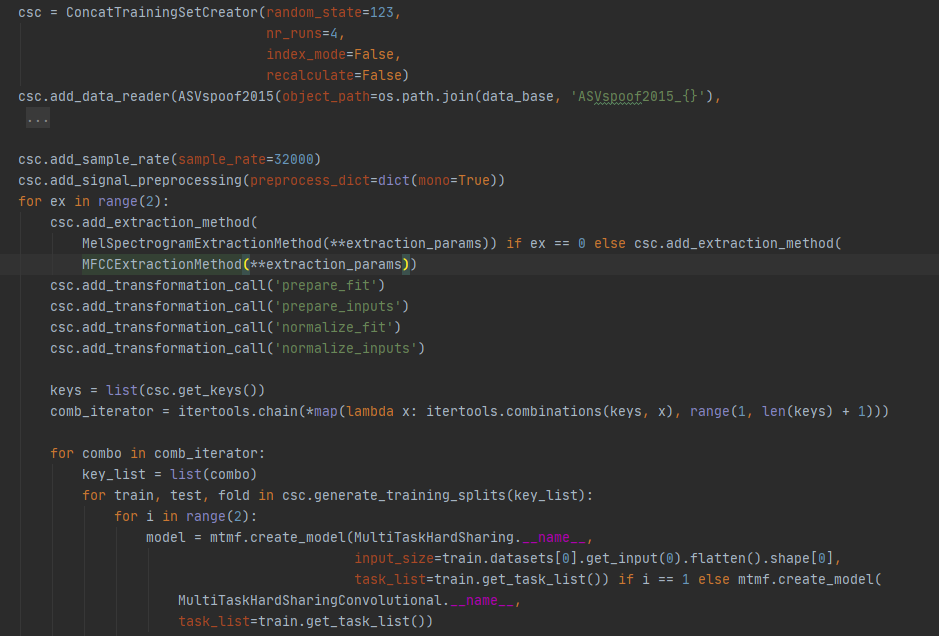
\includegraphics[width=\linewidth]{screenshot005}
	\caption{Data Loading in the variation experiments}
	\label{fig:screenshot005}
\end{figure}

In total 7 datasets were used in creating this set-up, with 8 tasks. The dataset linked to two tasks is the same used earlier for \citep{georgiev2017low}. The tasks contain both multi-class and multi-label tasks. Each combination is tested for 2 extraction methods and 2 models. For each run, the feature matrices should be framed in the same size, based on the average feature matrix size and the data normalized. As can be seen in table \ref{table:LOC}, this is the first time the required Training LOC makes a significant jump in the Training stage, simply due to the fact that it varies models. The models are loaded for the first time through the MultiTaskModel factory which mainly functions as a way to concentrate static and dynamic model parameters for creation and isn't absolutely necessary. Otherwise, the training is performed using the same three lines as before: model creation, results creation and training loop instantiation. The Data Loading stage also takes a jump, but is in no way related to the high and diverse amount of datasets, simply the variation of elements in the pipeline. There are  operations performed in the pipeline: resampling, conversion to mono, calculating and framing the feature matrices, normalizing the data. The Data loading code can be found in figure \ref{fig:screenshot005}, which makes it apparent that the extra lines outside the transformation calls are simply due to iterating over the required variations. The actual amount of LOC relating to direct data loading operations is 8.\\

This example makes it clear that all the work concerning datasets comes beforehand in the Data Reading stage, with little extra effort on the developer's side, while the combinatorial aspects are handled by the framework in the background. Nothing has to be explicitly reloaded or recalculated, as seen when adding the ExtractionMethod, by the developer as variations will be handled by the framework and necessary data recalculated when required. The framework thus reduces research variations to singular line changes.\\

To build on the last point of reducing work for research variations, especially in future work, it should be noted that given that the previous implementations would have been made as was the case in this scenario, only two extra datasets were added: FSD Kaggle 2018 TODO: REFERENCE and the Speech Commands dataset TODO: Reference. Given that, the Data Reading would be reduced to 8 + 83 LOC in this implementation. DataReader objects are merely paths for extracting the data, while the specifics of how can be given later. Vanilla implementations would either require large code changes if e.g. other extraction methods or signal preprocessing functions were required or have to take these in account beforehand and likely end up with similar structures. \\


\begin{figure}
	\centering
	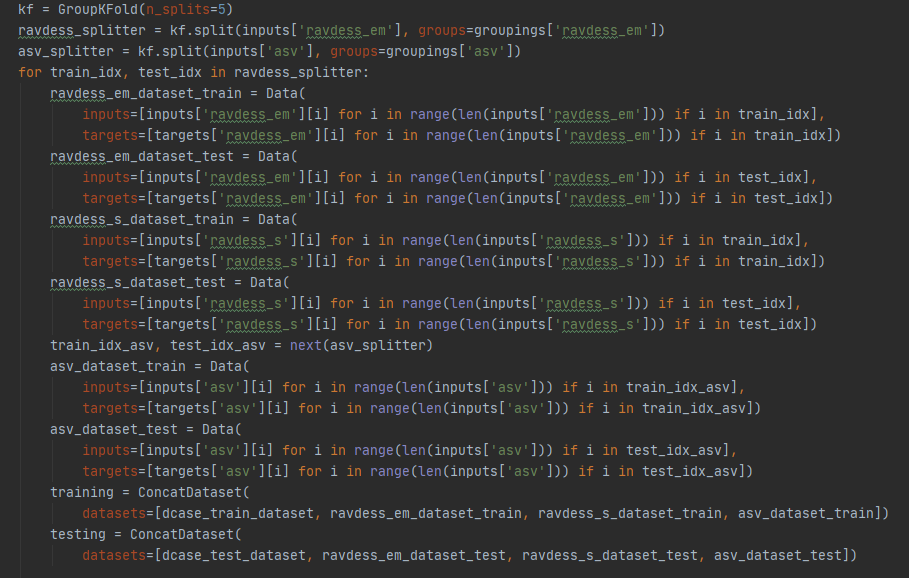
\includegraphics[width=\linewidth]{screenshot002}
	\caption{Train and Test set creation without framework for the \cite{georgiev2017low} implementation}
	\label{fig:screenshot002}
\end{figure}

\begin{figure}
	\centering
	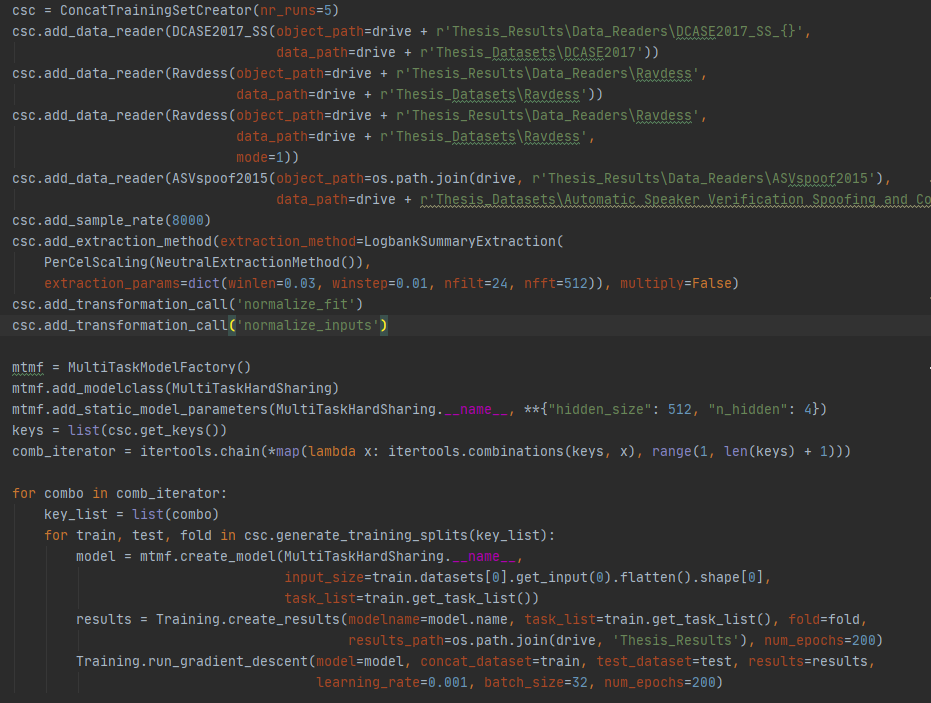
\includegraphics[width=\linewidth]{screenshot003}
	\caption{Complete implementation of \cite{georgiev2017low} with the framework}
	\label{fig:screenshot003}
\end{figure}

What these efforts demonstrate is that the LOC only directly scale with added required operations and do not spill over in other stages. To clarify the last part, figures \ref{fig:screenshot002} illustrate how without the framework, train and test set generation - which falls under the data loading stage - scales directly depending on the amount of datasets used. Compare that to figure \ref{fig:screenshot003}, where it can be seen that train and test generation is actually reduced to one simple line before the three Training stage lines in the end. This also demonstrates how the framework grants flexibility in which datasets to actually load and split with the key\_list input, which grants further work reduction as in practice it is possible that not all datasets are required which were planned beforehand. In the first case, that would imply multiple lines of code change, while in the second, simply one line for the key list. \\

What should again be noted, is that the implementations without the framework did not include a lot of the extra features that are performed automatically, the main one being quick reading and writing of the data. To reiterate, this means that when the Data Reading stage is done, it is written to files on the disk, so that future runs would not unnecessarily have to reextract feature matrices. Including these would raise the LOC required for the vanilla implementations a lot and would either have specific implementations per dataset or end up constructing similar functions to the framework. These LOC comparisons are for the bare required necessities only.\\



\begin{table}[ht]
	\caption{Reported metric comparisons} % title of Table
	\centering % used for centering table
	\begin{tabular}{p{0.25\textwidth}p{0.25\textwidth}p{0.25\textwidth}p{0.25\textwidth}} % centered columns (4 columns)
		\hline\hline %inserts double horizontal lines
		Title & Metric & Reported & Implementation  \\ [0.5ex] % inserts table
		%heading
		\hline % inserts single horizontal line
		\citet{park2020augmenting} & Precision & 0.796 & 0.7741 \\ \hline
		\citet{park2020augmenting} & Recall & 0.804 & 0.763  \\ \hline
		\citet{park2020augmenting} & F1 Score & 0.8 & 0.7685 \\ \hline
		\citet{georgiev2017low} & Accuracy Speaker Identification & 0.778 & 0.778 \\ \hline
		\citet{georgiev2017low} & Accuracy Emotion Recognition & 0.879 & 0.879 \\ \hline
		\citet{georgiev2017low} & Accuracy Stress Detection & 0.865 & 0.865 \\ \hline
		\citet{georgiev2017low} & Accuracy Ambient Scene Analysis & 0.825 & 0.825 \\ \hline
		\citet{xu2019multi} & Unweighted Average Recall & 0.662 & 0.6716 \\ \hline
	\end{tabular}
	\label{table:metric} % is used to refer this table in the text
\end{table}

Following the example from other deep learning frameworks like \cite{colacco2020drecpy} it is important that the framework demonstrates to be consistent with published results. In table \ref{table:metric} the comparative results can be found with the original publications. The decision was made to focus on the best reported performance of the multi-task setting, in order to limit the amount of work time to reproduce some of the results. Papers are often incomplete when it comes to specifics required to reproduce the same elements which can impact the results considerably, which requires careful variation and evaluation of the parameters.\\

Starting from the top, the results from the classifier built in \cite{park2020augmenting} come close but slightly below the reports. Multiple node amounts in the DNN were tried, as the original paper lacked to include the exact after the initial layer, yet implying the amount lessen through the figure included. Furthermore, the exact included instances are not the same. The work mentions some cleaning of the dataset was performed, but neglect to mention the specifics. The result is the best performing variation. The amount of nodes was halved in the final two layers and minimal logical clean up was performed (e.g. an audio fragment can not have both silence and another label at the same time). Still, the eventual results end up relatively close to the report.\\


\section{Literature Evaluation}

%TODO: Dive in the literature and describe its implementation on the software, which components can be adjusted or nah

\section{Fulfilment of the Requirements}

\subsection{Non-functional Requirements}
\begin{itemize}
	\item \textbf{Modular:} 
	%	Demonstrate the replaceability in the code
	\item \textbf{Extendible:} 
	%	Extensibility is discussed in design section
	\item \textbf{Fast prototyping:} 
	% Demonstration implementations, comparison with implementation without
	\item \textbf{Cutting Double Work:} 
	% Demonstration of the research set-up
%	\item \textbf{Developmental Side-rails:}
%	%  
	\item \textbf{Robust:} 
%	Demonstration + Dive in the literature

\end{itemize}

\subsection{Funtional Requirements}
\subsubsection{Data Reading}
\begin{itemize}
	\item Standardizing Input - The TaskDataset object is developed for assuring that the data is valid throughout the rest of the process. Its extension of PyTorch's Dataset class ensures that it can be utilised by the PyTorch framework. The builder pattern allows the TaskDataset to be built incrementally and valid along the way, with each step including various validity checks.
	The exception where the TaskDataset can't check for validity is in terms of the input feature matrix size. The matrix sizes might not be compatible with the developed PyTorch Model. The responsibility for this is up to the developer.
	% How do we know this works?
	% What validity checks?
	\item Handling dataset differences - The DataReader class is an abstract class that the developer must extend to deal with the peculiarities of navigating each dataset structure to extract the correct information. This corresponds to it being a white box hot-spot. Predefined train/test splits can be stored through the HoldTaskDataset structure and pre-split audio segments can be kept together by defining the grouping. 
	% Refer to the implementations for differences
	\item Scalable preprocessing - Preprocessing audio signals and preprocessing feature matrices happen in different places, as TaskDatasets should only contain valid input instances at any point. Preprocessing signals can utilise an (optional) function from the DataReader class with parameters that are received when the TaskDataset is extracted. Reusing the method can thus hand developers easy replicability of the signal preprocessing. These can be further scaled by using the TrainingSetCreator. In this class, any preprocessing or transformation can be added 'on the fly'. This means that if a functionality (e.g. resampling) is added, any previous 
	% What preprocessing do we have for both signals and feature matrices
	\item File storage abstraction: There are handles on the TaskDataset which can be called to store, load or check the TaskDataset to or from files, which are specific for the currently used extraction method and task.
	\item Quick Reading: The DataReader automatically checks if there is a stored TaskDataset available for the given extraction\_method and task and loads it if so.
	\item Create multiple input objects from the same dataset: (DEMONSTRATE) The framework is open ended in how the TaskDataset object is extracted from the data and allows extra parameters for the DataReader to be given at initialization. TaskDatasets are stored using the ExtractionMethod object's name and the (main) Task's name, so for every new variation of these will be automatically linked to different files.
	\item Tasks and datasets are a many to many relationship: Tasks can be present in multiple datasets. The tasks need to have the same name, output labels and classification type in order to be seen as the same. When combined in the ConcatTaskDataset, the target vectors will automatically be placed in the same positions, which will make them be seen as the same task in the training function. Datasets can have multiple tasks to an unlimited degree in its list of extra tasks, which always combines them with a list of targets of the same amount of input instances. 
\end{itemize}
\subsubsection{Data Loading}
\begin{itemize}
	\item Combining datasets: Extended the ConcatTaskDataset, extra functions for the batching
	\item Not requiring the combined datasets in memory:  Index mode implemented which forms a streaming context for the data to be stored and read from disk.
	\item Train and test set generation: They implemented through the HoldTaskDataset
	\item Transforming data: They implemented through handles on the TaskDataset which call upon the ExtractionMethod
	\item Filtering data: Handle on the TaskDataset
	\item Reusing data: It implemented, reusability is possible without reloading to different degrees
	\item Batching multiple tasks: It implemented lol
	\item Replicability: It implemented through storing the different checkpoints (which can be recreated by reloading the Results object), the calculation data in extractionmethods and 
	\item Scalable Manipulation: In the TrainingSetCreator, manipulations can be added for one specified dataset or all at once.
\end{itemize}
\subsubsection{Training}
\begin{itemize}
	\item Predicting multiple tasks: Each dataset can have multiple tasks linked to their targets. There are automatic filters for the output to isolate the task specific predictions. 
	\item Task specific output handling: Handling of the task functions, like loss calculation and decision making of the eventual classes from the probabilities are stored in the Task objects 
	\item Loss calculation specifiable: The calculation of the Loss of each task is definable in the Task object. However, currently, losses are always tied to tasks, which have target labels. This is not always the case, as in the research \citep{tagliasacchi2020multi} \citep{wu2020domain}, losses have also been calculated based on cost functions from internal model parameters. Since these loss functions are not linked to datasets, but to the models themselves, for which the framework does not offer modules which can be used in the training function for specific handling, it is up to the developer to implement these in the Training\_Utils object.
	\item Loss combination specifiable: Implemented in the Training\_Utils object
	\item Metric calculation, storage and visualization: Gives predictions, true labels and losses to the Results object which calculates the metrics, stores them and writes them to tensorboard where they can easily be compared to other results
	\item Interrupted Learning: (DEMONSTRATE) Implemented by recreating the Results object and starting the training loop from the given epoch.
	\item Separate evaluation: (DEMONSTRATE) The evaluation function is separate from the training loop. Training parameters for transformations and such can be reloaded from the stored extraction\_method object as well as the model parameters at every epoch in the training function. 
	\item Direct comparison of different runs: Every run has a unique name and TensorBoard has the ability to place the results from different files side-by-side
	\item Variable training paradigms: In this state, the only training paradigm available is Gradient Descent. Implementing a different paradigm requires foregoing the current training loop implementation.
\end{itemize}